\documentclass[12pt,a4paper]{article} % 使用article文档类,字体大小为12pt,纸张为A4

% 引入必要的包
\usepackage[UTF8]{ctex} % 支持中文
\usepackage{amsmath} % 数学公式
\usepackage{amssymb} % 数学符号
\usepackage{geometry} % 设置页面边距
\usepackage{graphicx} % 插入图片
\usepackage{listings} % 插入代码
\usepackage{xcolor} % 自定义颜色
\usepackage{booktabs} % 表格优化
\usepackage{enumitem} % 调整列表格式
\usepackage[backref, colorlinks,linkcolor=blue]{hyperref}

% 页面设置
\geometry{left=2.5cm,right=2.5cm,top=2.5cm,bottom=2.5cm} % 设置页边距

% 代码样式设置
\lstset{
    basicstyle=\ttfamily\small, % 设置代码字体和大小
    numbers=left, % 显示行号
    numberstyle=\tiny, % 行号字体
    keywordstyle=\color{blue}, % 关键词颜色
    commentstyle=\color{gray}, % 注释颜色
    stringstyle=\color{red}, % 字符串颜色
    breaklines=true, % 自动换行
    frame=single, % 添加边框
    backgroundcolor=\color{gray!10} % 背景颜色
}

\title{随手记} % 文档标题
\author{王成} % 作者
\date{\today} % 日期

\begin{document}

\maketitle % 生成标题

\section{知乎}
\subsection{集总参数模型中的地解释}
\colorbox{yellow!20}{
    \parbox{\dimexpr\linewidth-2\fboxsep}{
        由于血液从心脏射出,流经动脉,然后进入毛细血管和静脉系统,流回到心脏。在电网络模型中,可以将心脏视为交流电源。由于静脉系统的血压较低,可以将静脉视为零电位,血液流入静脉视为电路中的“接地”。动脉系统的整体电网络模型如图所示:
    }
}

\section{叙述性内容}
\subsection{本课题的研究内容及意义}
本课题主要针对缺血性脑卒中患者的治疗,通常在患者中风后被送往医院的4.5\textasciitilde6小时内,先通过CT,MRI等影像技术对血管狭窄或阻塞部位进行快速定位,然后基于该部位制定合适的手术如动脉机械取栓(EVT)或者静脉溶栓(IVT)等。
由于缺血性卒中的治疗具有时间敏感性,延迟会显著影响预后,如脑组织和神经系统因缺血缺氧而死亡凋零,致使患者残疾或死亡,于是在患者通过手术血管再通后,需要辅以自体血低温脑灌注,以降低脑部新陈代谢速率,减少脑细胞死亡速率,延长治疗时间窗,挽救缺血半暗带,降低患者致死致残率。

\subsection{动脉顺应性与静脉顺应性}
    静脉顺应性通常是动脉顺应性的10\textendash 20倍,因此,当动脉血管内血液量减少而静脉血管内血液量增加时,动脉压的下降幅度通常至少是静脉压上升幅度的 10 倍。

    静脉压力-容积关系的非线性特性了用如下关系表示:
\begin{equation*}
    \Delta V = \frac{2 \cdot \Delta V}{\pi} \arctan \left( \frac{\pi \cdot C_0}{2 \cdot \Delta V_{\text{max}}} \cdot \Delta P_{\text{trans}} \right)
\end{equation*}
其中,$\Delta V$表示跨壁压引起的腔室容积变化量,$\Delta V_{\text{max}}$ 表示腔室容积最大变化量,$C_0$表示基础跨壁压,即$\Delta P_{\text{trans}} = 0$ 时的腔室顺应性。下图 \ref{fig:nonlinear-compliance} 展示了非线性静脉顺应性的压力-容积关系曲线。
\begin{figure}[htbp]
    \centering
    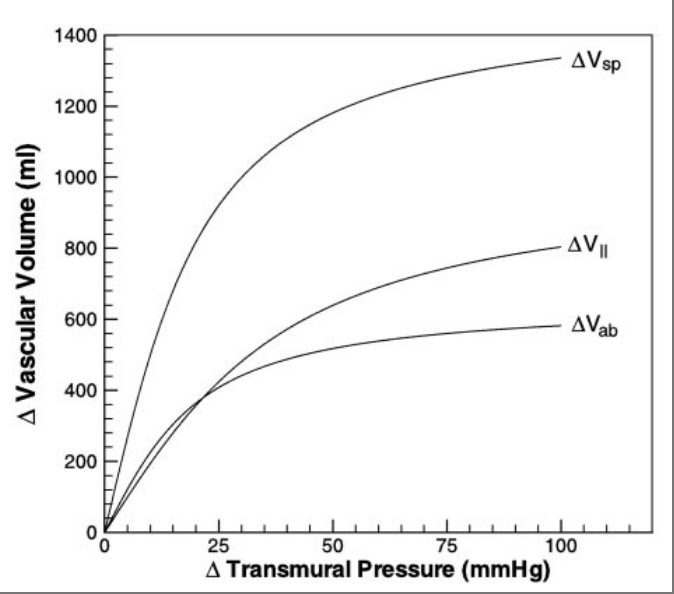
\includegraphics[width=0.6\textwidth]{figures/非线性顺应性.png}
    \caption{Pressure-volume relations for changes in stressed volume of the abdominal ($ V_{ab}$), leg ($V_{ll}$), and splanchnic ($V_{sp}$) venous compartments.}
    \label{fig:nonlinear-compliance}
\end{figure}
具体建模方法与内容可参考文献如下\cite{heldtComputationalModelingCardiovascular2002}。

\subsection{动脉血二氧化碳}
动脉血中二氧化碳浓度的变化对脑总血流量有重要影响。高碳酸血症会扩张脑血管并增加血流量,而低碳酸血症则会收缩脑血管并减少血流量。血氧含量的变化会产生相反效果,但其引发的血管收缩或扩张刺激作用弱于血二氧化碳浓度的变化\cite{pina-garzaChapter4Increased2013}。

颅内结构对缓慢增加的压力适应能力相当强,但突然的变化则无法耐受,会导致头痛、性格改变和意识水平下降等不同症状的组合。

\subsection{治疗性低温}
低温会降低脑血流量。将体温维持在27°C至31°C之间最为理想。除其他降低脑血流量的措施外,低温疗法的额外获益尚不明确\cite{pina-garzaChapter4Increased2013}。

治疗性低温通过改变血管直径来实现对脑血流量的影响。低温会导致血管收缩,降低脑血流量。通过实验观测得到了治疗性低温对血管直径调控的理论模型\cite{josephUsingHumanCirculation2022,konstasTheoreticalModelSelective2007}。
\begin{equation*}
    D_{35.5} = D_{37.5} \times Q_{10}^{\beta(35.5-37.5)}
\end{equation*}
其中$D_T$表示温度T时的血管直径,$Q_{10} = 2.96$,$\beta = 0.08$ \cite{josephUsingHumanCirculation2022}。随后利用这些直径数据重新分配模型中的所有阻力值。

\bibliographystyle{plain}
\bibliography{Bible/ref} % 参考文献文件名
\end{document}